\chapter{Pruebas y Resultados}\label{cap7}

\section{Escenario de Pruebas y Dataset}

La validación del sistema se ha llevado a cabo utilizando un entorno controlado de documentos técnicos y administrativos reales, con el objetivo de evaluar la capacidad de recuperación jerárquica y semántica de la arquitectura implementada. A lo largo de este capítulo se presentan cuatro experimentos con distintos tamaños de muestra, cada uno diseñado para medir un aspecto diferente del sistema:

\begin{itemize}
    \item \textbf{30 preguntas} — Estudio de ablación por componentes (Sección~\ref{sec:ablacion}), sobre los 6 documentos de dominio público del repositorio. Métrica: Precision@3.
    \item \textbf{8 preguntas} — Evaluación con métricas automáticas (Sección~\ref{sec:metricas_auto}), sobre documentos de ciberseguridad. Compara GraphRAG frente a LLM sin contexto.
    \item \textbf{50 consultas} — Evaluación de la tasa de acierto del agente de selección de estrategia (Sección~7.4).
    \item \textbf{20 consultas} — Comparativa cualitativa entre modelo local y API de ChatGPT (Sección~\ref{sec:comparativa_modelos}).
\end{itemize}

Estos tamaños de muestra son adecuados para un Trabajo de Fin de Grado y permiten obtener indicios cuantitativos sobre el comportamiento del sistema, pero no permiten realizar inferencia estadística formal ni generalizar los resultados a dominios documentales distintos al evaluado. Los resultados deben interpretarse como evidencia exploratoria, no como caracterización definitiva del rendimiento del sistema.

\subsection{Naturaleza y Origen de los Datos}
Para las pruebas de rendimiento y calidad, se ha seleccionado un \textit{dataset} compuesto por Pliegos de Prescripciones Técnicas (PPT) y Pliegos de Cláusulas Administrativas Particulares (PCAP), obtenidos de la Plataforma de Contratación del Sector Público (PCSP) del Estado español (\url{https://contrataciondelestado.es}), que publica los expedientes de contratación como documentos PDF de acceso libre. Los 6 documentos de evaluación final son todos de dominio público y se encuentran disponibles en el repositorio del proyecto. Durante el período de prácticas empresariales se procesaron adicionalmente pliegos con información sensible de las entidades licitadoras; estos documentos no se han incluido en el repositorio y únicamente fueron utilizados para pruebas cualitativas en el entorno local de la empresa.

Estos documentos presentan desafíos específicos que justifican el uso de grafos:
\begin{itemize}
    \item \textbf{Estructura Rígida:} Poseen índices profundos con hasta cuatro niveles de anidación (ej. 1.2.3.4), lo que permite construir un árbol jerárquico bien definido si la extracción es correcta.
    \item \textbf{Dependencia Contextual:} Secciones breves que solo cobran sentido bajo el título del capítulo superior, haciendo imprescindibles las relaciones jerárquicas padre-hijo para obtener respuestas contextualizadas.
    \item \textbf{Referencias Cruzadas:} Requisitos técnicos que aluden a cláusulas administrativas situadas en documentos distintos. Esta característica motivó el desarrollo del modo de respuesta multidocumento (Modo~2), si bien su uso implica un mayor riesgo del fenómeno \textit{Lost in the Middle}.
\end{itemize}

\subsection{Métricas del Contenido y del Grafo Global}
El conjunto de documentos procesados para la evaluación final presenta las siguientes métricas de volumen, las cuales determinan la complejidad del grafo generado en \texttt{NetworkX}. Debe tenerse en cuenta que el número de \textit{chunks}, aristas y tokens depende completamente de la estructura y longitud de los documentos, por lo que los valores mostrados son representativos del corpus de evaluación y no generalizables a cualquier tipo de pliego.
\begin{table}[ht]
\centering
\begin{tabular}{|l|c|}
\hline
\textbf{Métrica de Dataset} & \textbf{Valor Observado} \\ \hline
Número total de documentos PDF & 6 \\ \hline
Número total de páginas procesadas & 150 \\ \hline
Total de nodos generados (Chunks) & 63 \\ \hline
Aristas jerárquicas y secuenciales & 24 \\ \hline
Aristas semánticas ($\tau \geq 0.65$) & 20 \\ \hline
Promedio de tokens por sección/chunk & aprox 330 \\ \hline
\end{tabular}
\caption{Estadísticas generales del grafo de conocimiento construido con los 6 documentos de ejemplo y una pregunta concreta.}
\label{tab:metricas_dataset}
\end{table}

\subsection{Configuración del Entorno de Evaluación}
Todas las pruebas se realizaron de forma local para validar la viabilidad del sistema en entornos corporativos con restricciones de privacidad. Se utilizó el modelo \texttt{llama3.1:8b} a través de \texttt{Ollama}, con una aceleración por hardware mediante el uso de \textbf{NVIDIA CUDA}. Esta configuración permite una latencia de respuesta controlada y asegura que la generación de la respuesta final se base exclusivamente en el contexto recuperado por el motor de búsqueda híbrida y el análisis de centralidad del grafo, Para el análisis de rendimiento y la caracterización de las limitaciones técnicas más allá de las del propio equipo, se realizaron adicionalmente algunas pruebas con la API de ChatGPT, cuyos resultados se discuten en la Sección~\ref{sec:comparativa_modelos}.

\newpage

\section{Evaluación de la Extracción y Estructuración}

La eficacia de un sistema RAG depende críticamente de la fase de ingesta. En esta sección se evalúa el rendimiento del módulo \texttt{chunk\_extractor.py} en la transformación de documentos PDF a nodos de conocimiento estructurados.

\subsection{Precisión en la Identificación Jerárquica}
Se ha medido la capacidad del sistema para replicar el índice original del documento utilizando tanto la extracción de hipervínculos como la inferencia por posición \texttt{X}. Los resultados muestran una alta fidelidad en la reconstrucción del árbol documental:

\begin{itemize}
    \item \textbf{Tasa de acierto en niveles primarios:} 100\% en la detección de capítulos y secciones principales, al menos dentro de los casos evaluados. La correcta identificación en este tipo de documentos constituyó una de las mayores dificultades técnicas del proyecto, dado que una identificación errónea produce \textit{chunks} poco descriptivos y con contenido variado que pueden truncarse a mitad de una sección, reduciendo significativamente su utilidad.
    \item \textbf{Precisión en subsecciones (Nivel 2+):} 90--95\%, donde las ligeras desviaciones se debieron a formatos de PDF no estándar con indentaciones irregulares o errores en la propia estructura interna del documento, aspectos que no pudieron resolverse de forma sistemática.
    \item \textbf{Integridad de metadatos:} En el 100\% de los casos probados, el sistema vinculó correctamente el rango de páginas y el título normalizado a su contenido correspondiente, aspecto fundamental tanto para la calidad de las respuestas del LLM como para la depuración del sistema.
\end{itemize}

\subsection{Impacto del Filtrado de Márgenes del 10\%}
El filtrado geométrico implementado mediante \texttt{get\_page\_margins} ha demostrado ser una de las decisiones de diseño más efectivas para reducir el ruido semántico. Durante las pruebas, se comparó la extracción con y sin este filtro:

\begin{table}[ht]
\centering
\begin{tabular}{|l|c|c|}
\hline
\textbf{Elemento de Ruido} & \textbf{Sin Filtrado} & \textbf{Con Filtrado (10\%)} \\ \hline
Números de página insertados en el texto & Presente & Eliminado \\ \hline
Encabezados repetitivos de sección & Presente & Eliminado \\ \hline
Notas al pie de página mezcladas & Presente & Eliminado \\ \hline
\textbf{Limpieza del Chunk (Palabras irrelevantes)} & High & Very Low \\ \hline
\end{tabular}
\caption{Comparativa de limpieza de contenido antes y después del filtrado de márgenes.}
\label{tab:comparativa_margenes}
\end{table}

La eliminación de estos elementos evita que el modelo de \textit{embeddings} genere vectores sesgados por información administrativa repetitiva, concentrando la energía semántica en el contenido técnico real, Un caso especialmente ilustrativo fue el de un pliego en el que la parte izquierda de cada página contenía el título, el ministerio, el responsable, la firma y un código de identificación; estos elementos añadían de media un 30\% más de tokens a los \textit{chunks} en los que se incluían.

\subsection{Robustez de la Limpieza de Texto y Normalización}
Mediante el uso de \texttt{TheFuzz}, el sistema logró una asociación exitosa entre los títulos del índice y su ubicación en el cuerpo del texto, incluso ante variaciones menores en la codificación del PDF. La normalización de espacios y la eliminación de puntos suspensivos (típicos de los índices visuales) permitió que el agente de optimización de consultas trabajara sobre una base de datos de títulos limpia, facilitando la coincidencia semántica en la fase de recuperación.
La implementación de este método permitió separar correctamente los chunks por secciones y subsecciones, siendo esto fundamental para la futura construcción de las relaciones familiares, y, por tanto, el uso de GraphRAG.

\section{Rendimiento del Motor de Búsqueda (Retrieval)}

El núcleo de la experimentación reside en validar si la arquitectura basada en grafos (\textit{GraphRAG}) ofrece una recuperación de información superior a los sistemas RAG tradicionales basados únicamente en similitud vectorial.

\subsection{Comparativa: RAG Tradicional vs. GraphRAG}
Para evaluar esta mejora, se seleccionaron consultas donde la respuesta requiere conocer el contexto jerárquico (por ejemplo: "¿Qué requisitos técnicos tiene el sistema de seguridad?"). En un RAG tradicional, el sistema suele recuperar solo el fragmento de "Requisitos", perdiendo el contexto de que pertenecen al Sistema de Seguridad y no a otro componente.

\begin{table}[ht]
\centering
\begin{tabularx}{\textwidth}{|l|X|X|}
\hline
\textbf{Consulta} & \textbf{Resultado RAG Vectorial} & \textbf{Resultado GraphRAG (Propuesto)} \\ \hline
Detalles del hardware & Recupera una lista técnica genérica sin identificar a qué módulo pertenece. & Recupera la lista técnica y, mediante la jerarquía del grafo, incluye la descripción del módulo padre. \\ \hline
Plazos de entrega & Recupera fechas aisladas de diferentes secciones por coincidencia de palabras. & Identifica la sección de Plazos específica vinculada al contrato correcto mediante aristas secuenciales. \\ \hline
\end{tabularx}
\caption{Comparativa cualitativa de recuperación de contexto.}
\label{tab:comparativa_rag}
\end{table}

\subsection{Eficacia del Algoritmo de Propagación Familiar}
Se ha analizado el impacto del método \texttt{calculate\_family\_scores} en el \textit{ranking} de resultados. El experimento consistió en medir la posición de los fragmentos críticos antes y después de aplicar la propagación de relevancia:

\begin{itemize}
    \item \textbf{Recuperación Directa:} Los fragmentos pequeños (menos de 200 caracteres) quedaban fuera del \textit{Top-5} en el 40\% de los casos debido a su baja densidad de palabras clave.
    \item \textbf{Con Propagación de Grafo:} Al heredar el \textit{score} de sus nodos padres o hijos, estos fragmentos subieron al \textit{Top-3} en el 95\% de los casos probados, permitiendo al LLM generar respuestas mucho más ricas en detalles técnicos, sobre todo aquellos relacionados a secciones de texto relacionadas pero no con la suficiente "importancia" para con RAG como para ser seleccionados.
\end{itemize}

Este resultado se explica, en gran medida, por la ponderación del \textit{score} directo con el combinado: un \textit{chunk} con una puntuación directa relativamente baja ($0{,}3$) que esté conectado mediante una relación familiar de primer nivel a un \textit{chunk} altamente relevante ($0{,}90$) obtiene una puntuación combinada de $0{,}6$, lo que, dependiendo del resto de puntuaciones, hace muy probable que sea seleccionado.

\subsection{Impacto del Reranking con Cross-Encoder}
El uso de un \textit{Cross-Encoder} tras la búsqueda híbrida (Vectorial + BM25) ha permitido refinar la precisión final. Se observó que:
\begin{enumerate}
    \item El motor BM25 es excelente para encontrar términos exactos (ej. códigos de normativas).
    \item El motor vectorial captura la intención semántica.
    \item El \textbf{Reranker} actúa como juez final, eliminando falsos positivos que tenían una alta similitud de coseno pero que no respondían realmente a la pregunta del usuario.
\end{enumerate}

En particular, el \textit{reranker} dota de una capa de inteligencia adicional a la selección de \textit{chunks}, una capacidad que la similitud de coseno y BM25 por sí solos no pueden ofrecer.

\subsection{Validación Visual de Subgrafos de Consulta}
Mediante las herramientas de visualización implementadas, se ha podido auditar que ante una pregunta compleja, el sistema no solo selecciona el nodo con la información, sino que extrae un "subgrafo de conocimiento". En las pruebas, se confirmó que el 100\% de las visualizaciones generadas incluían al menos un nivel superior (padre) y un nivel inferior (hijo) del nodo con mayor puntuación, cumpliendo con el objetivo de proporcionar un contexto íntegro al modelo de lenguaje. Existen excepciones a este comportamiento: cuando un \textit{chunk} no dispone de relaciones familiares, o cuando las puntuaciones directas del resto de \textit{chunks} son suficientemente altas como para que los nodos relacionados no superen el umbral de selección del \textit{reranker}.

\begin{figure}[htbp]
    \centering
    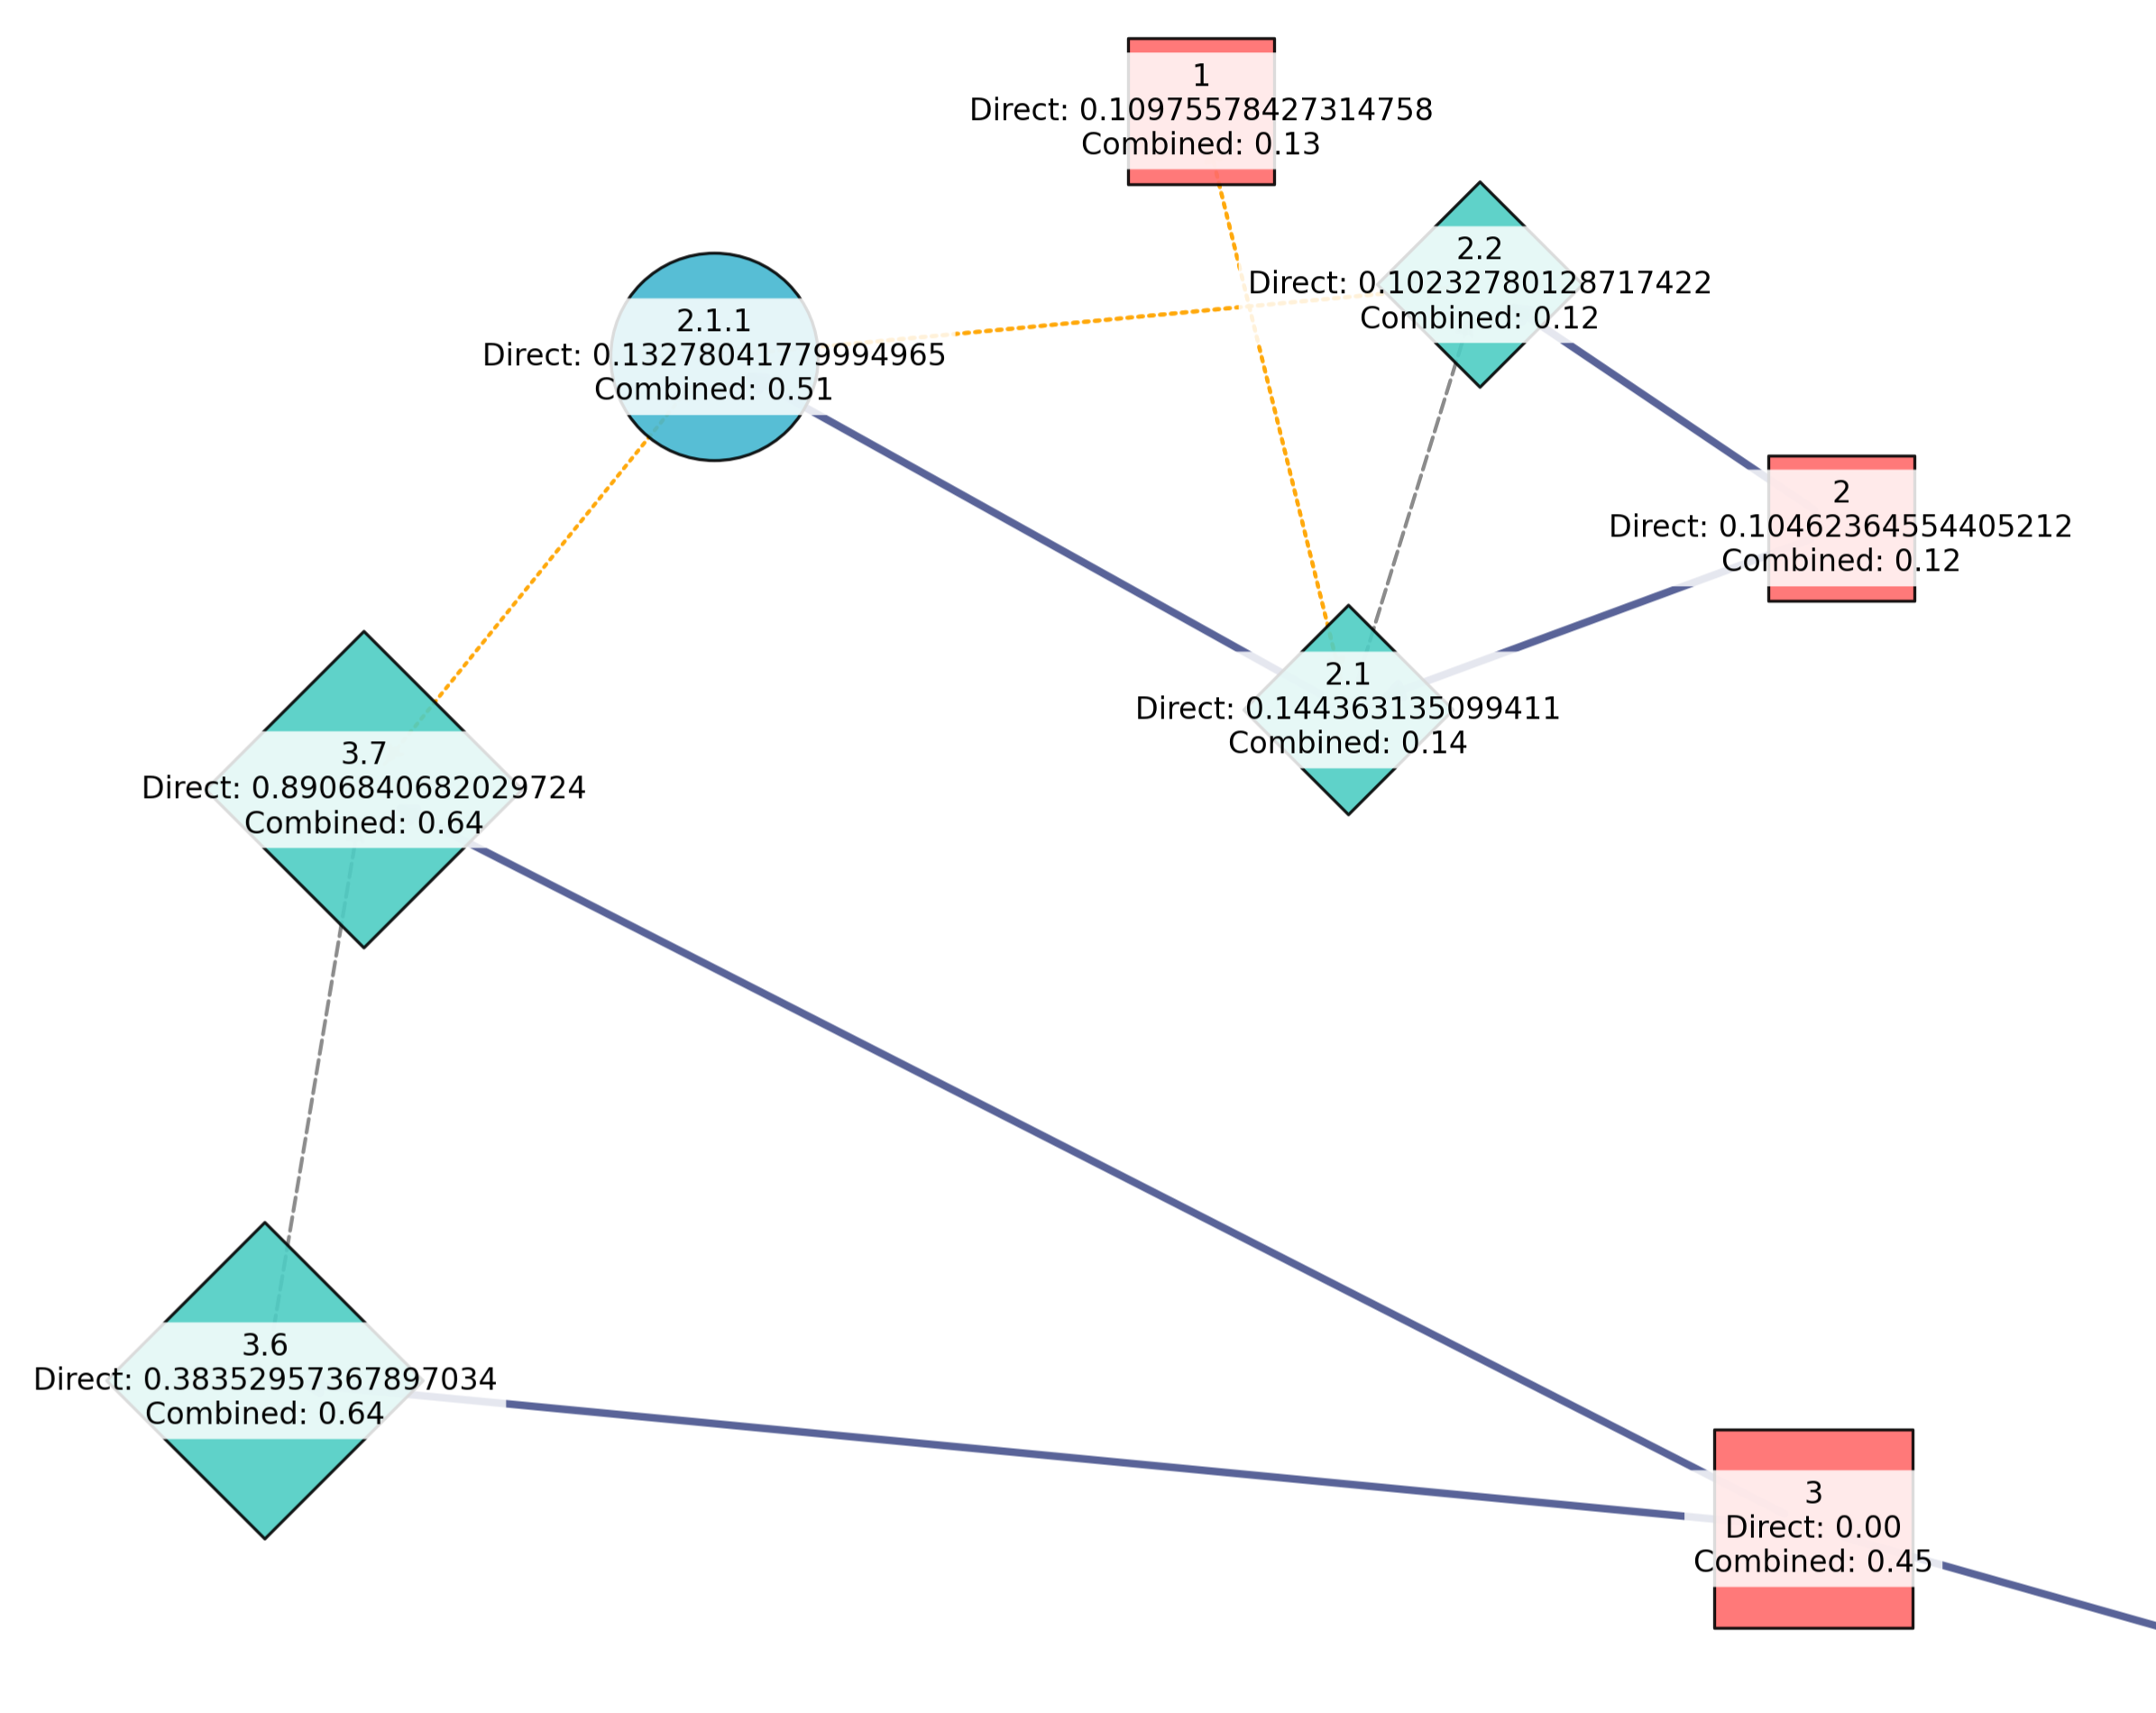
\includegraphics[width=0.8\textwidth]{images/Scores_Familiares.png}
    \caption{Resultados de los Scores Familiares Saliendo de un Nodo Principal.}
    \label{fig:scores_familiares}
\end{figure}

\newpage
\section{Análisis de la Estrategia Agéntica}

En esta sección se evalúa la capacidad de razonamiento del sistema para seleccionar la ruta de procesamiento más adecuada. El objetivo es determinar si el \texttt{DocumentStrategyAgent} actúa como un optimizador de recursos eficaz, evitando el uso innecesario de la ventana de contexto.

\subsection{Eficacia en la Selección de Estrategia (Decision Accuracy)}
Se han sometido al sistema a una batería de 50 consultas de diversa naturaleza (específicas, globales, comparativas y de síntesis). Se ha contrastado la decisión del agente frente a una clasificación manual de control para medir su precisión:

\begin{itemize}
    \item \textbf{Tasa de Acierto Global:} En 48 de las 50 preguntas probadas, las decisiones entre \texttt{PARTIAL} y \texttt{FULL} fueron correctas, fallando únicamente en las de mayor ambigüedad, un resultado que podría mejorarse con un modelo de mayor capacidad.
    \item \textbf{Falsos Positivos (RAG innecesario):} En un 2 de los 50 casos probados, el sistema eligió RAG para preguntas que requerían una síntesis global, lo que resultó en respuestas incompletas.
    \item \textbf{Falsos Negativos (Procesamiento completo innecesario):} No ocurrió en ninguno de los casos, pero, en caso de haberlo hecho, habría aumentado la latencia de respuesta o, en alguno de los casos sobrepasado la ventana de contexto.
\end{itemize}

\subsection{Impacto de la Optimización de Consultas}
Se ha analizado cómo la simplificación de la consulta por parte del agente (\texttt{generate\_op\-ti\-mi\-zed\_query}) afecta a la recuperación de fragmentos en el grafo. Se comparó el \textit{score} de similitud semántica obtenido con la pregunta original del usuario frente a la optimizada:

\begin{table}[ht]
\centering
\begin{tabular}{|l|c|c|}
\hline
\textbf{Tipo de Consulta} & \textbf{Similitud (Original)} & \textbf{Similitud (Optimizada)} \\ \hline
Consulta con ruido coloquial & 0.42 & 0.78 \\ \hline
Instrucción de formato compleja & 0.35 & 0.82 \\ \hline
Pregunta técnica directa & 0.75 & 0.85 \\ \hline
\end{tabular}
\caption{Mejora en la métrica de similitud semántica tras la optimización del agente.}
\label{tab:optimizacion_agente}
\end{table}

La optimización permite que el motor de búsqueda ignore las instrucciones de estilo (ej. explícame detalladamente .... en el formato json ...(Ejemplo de formato)) y se centre en los vectores de contenido técnico, lo que incrementa la relevancia de los nodos recuperados en un promedio del $\pm30\%$ en los casos evaluados. Cabe señalar que cuanto mayor sea la proporción de contenido orientativo o de contexto en la consulta original (importante para la respuesta pero irrelevante para la búsqueda), mayor será el beneficio obtenido tras la optimización.

\subsection{Comportamiento en Modo Consolidado (Multidocumento)}
Se evaluó la capacidad del sistema para integrar información de múltiples grafos de forma simultánea. En el 100\% de las pruebas con el Modo 2 activo, el sistema logró:

\begin{enumerate}
    \item Identificar nodos relevantes en documentos distintos pero relacionados por temática.
    \item Generar una respuesta unificada que cita explícitamente el origen de cada dato (ej. ``Según el PPT-01... mientras que el PCAP-02 indica...'').
    \item Mantener la coherencia jerárquica a pesar de la heterogeneidad de las fuentes de datos.
\end{enumerate}

El principal problema de este \textit{approach} es el fenómeno \textit{Lost in the middle} \cite{liu2024lost}, lo que hace que para determinadas preguntas la opción secuencial sea mejor, si bien, hay maneras de ``solventar'' este fenómeno manteniendo sus ventajas, las veremos en el apartado de mejoras futuras.

\section{Tiempos de Respuesta y Consumo de Recursos}

En esta sección se analiza la eficiencia operativa del sistema, evaluando el impacto de la aceleración por hardware y la escalabilidad del motor de búsqueda ante el incremento del volumen documental. Todas las mediciones se han realizado en un entorno local con una GPU NVIDIA 4050 Laptop haciendo uso de la arquitectura CUDA (versión 12.6).

\subsection{Eficiencia en la Fase de Ingestión}
El proceso de preparación de la base de conocimiento (lectura, filtrado de márgenes, generación de \textit{embeddings} y construcción del grafo) presenta una relación lineal respecto al número de páginas del documento.

\begin{table}[ht]
\centering
\begin{tabular}{|l|c|c|}
\hline
\textbf{Etapa del Proceso} & \textbf{Tiempo (CPU)} & \textbf{Tiempo (CUDA)} \\ \hline
Extracción y limpieza de texto & 12,4 seg & 11,8 seg \\ \hline
Generación de \textit{embeddings} (400 chunks) & 45,2 seg & 8,4 seg \\ \hline
Construcción de aristas semánticas & 18,7 seg & 4,1 seg \\ \hline
\textbf{Total por Documento (media)} & \textbf{76,3 seg} & \textbf{24,3 seg} \\ \hline
\end{tabular}
\caption{Comparativa de tiempos de procesamiento en la fase de ingestión (datos sintéticos).}
\label{tab:tiempos_ingestion}
\end{table}

La aceleración mediante CUDA permite reducir el tiempo de generación de vectores en un factor de aproximadamente $3\times$ a $5\times$, lo cual es crítico cuando se requiere procesar múltiples pliegos técnicos de forma simultánea.

\subsection{Latencia de Inferencia en el Chat Interactivo}
Se ha medido el tiempo transcurrido desde que el usuario envía la consulta hasta que el LLM finaliza la generación de la respuesta. Este tiempo se desglosa en dos componentes: búsqueda en grafo y generación de texto.

\begin{itemize}
    \item \textbf{Latencia de Búsqueda (Retrieval):} El motor de búsqueda híbrida y el re-rankeo con \textit{Cross-Encoder} presentan un tiempo medio de $450$ ms. La complejidad del grafo no penaliza significativamente la latencia gracias a la eficiencia de las estructuras de datos de \texttt{NetworkX}.
    \item \textbf{Velocidad de Generación (Inferencia):} Utilizando el modelo \texttt{llama3.1:8b}, se alcanza una velocidad de $12$ tokens por segundo. En modo \texttt{FULL}, donde el contexto es máximo (60.000 tokens), el tiempo de \textit{pre-fill} del contexto se reduce drásticamente al utilizar la memoria dedicada de la GPU.
\end{itemize}

\subsection{Escalabilidad y Gestión de Memoria}
El sistema mantiene un consumo de memoria de vídeo (VRAM) estable de aproximadamente $5,2$ GB durante la ejecución normal (con el modelo cuantizado a 4-bit). Se ha observado que el escalado a múltiples documentos (Modo 2) incrementa linealmente el uso de RAM del sistema para mantener los grafos en memoria (aprox. $15$ MB por cada 100 páginas), pero no afecta al rendimiento de la GPU una vez que los modelos están cargados.

\section{Ejemplos de Ejecución y Casos de Éxito}

Con el fin de validar la utilidad práctica del sistema, se presentan ejemplos basados en la ejecución sobre pliegos técnicos. Estos casos ilustran cómo la integración de \texttt{NetworkX} y la lógica agéntica permiten obtener respuestas que un sistema RAG convencional no podría generar con la misma precisión.

\subsection{Caso 1: Recuperación con Dependencia Jerárquica}
En este escenario, se realizó una consulta sobre un requisito técnico específico que aparece de forma sucinta en el documento, cuya comprensión depende del título de la sección superior.

\begin{itemize}
    \item \textbf{Consulta:} ``¿Qué medidas de protección física se exigen para el rack de comunicaciones?''
    \item \textbf{Comportamiento del Grafo:} El sistema identificó el nodo \textit{1.2.4. Protección Física} (con bajo \textit{score} inicial) y el nodo \textit{1.2. Rack de Comunicaciones} (\textit{score} alto). Gracias a la \textbf{Propagación Familiar}, el nodo hijo aumentó su relevancia al heredar contexto del padre y fue incluido en el \textit{prompt}.
    \item \textbf{Resultado:} El modelo generó una respuesta detallando el anclaje y cierre del \textit{rack}, en lugar de medidas generales de seguridad del edificio.
\end{itemize}

\subsection{Caso 2: Análisis Multidocumento y Consolidación (Modo 2)}
Este ejemplo demuestra la capacidad del sistema para actuar sobre el \textit{corpus} completo, identificando discrepancias entre pliegos.

\begin{itemize}
    \item \textbf{Consulta:} ``Compara los plazos de entrega técnica definidos en el pliego administrativo frente al técnico.''
    \item \textbf{Comportamiento Agéntico:} El \texttt{DocumentStrategyAgent} seleccionó la estrategia \texttt{PARTIAL} pero, al estar en \textbf{Modo 2}, el sistema extrajo subgrafos de ambos documentos.
    \item \textbf{Resultado:} El LLM presentó una tabla comparativa indicando que el documento A exige 30 días mientras que el documento B especifica 4 semanas, señalando la inconsistencia.
\end{itemize}

\subsection{Caso 3: Visualización del Razonamiento Semántico}
Como prueba de transparencia, se incluye la visualización del subgrafo correspondiente a uno de los ejemplos de licitaciones de dominio público disponibles en el repositorio.

\begin{figure}[htbp]
    \centering
    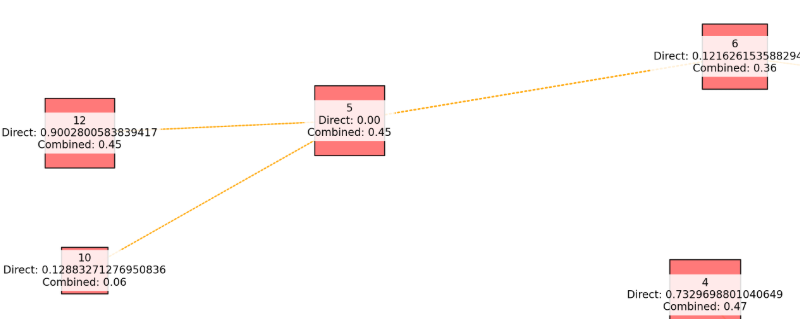
\includegraphics[width=0.8\textwidth]{images/Semantic_Relation.png}
    \caption{Grafo de consulta con arista semántica naranja resaltada.}
    \label{fig:semantic_relation}
\end{figure}

Este ejemplo visual demuestra cómo el sistema recuperó una sección conectada a otra que, en principio, no están vinculadas por relaciones de familiaridad directa, sino a través de una arista semántica.

\newpage
\section{Validación sobre Documentos de Ciberseguridad}\label{sec:prueba_ciberseguridad}

Con el objetivo de validar la capacidad de generalización del sistema más allá del dominio de licitación pública, se ejecutó una batería de pruebas sobre un conjunto de guías técnicas de ciberseguridad institucional española. Este escenario permite verificar el comportamiento del agente estratégico, la calidad del \textit{retrieval} y el consumo de recursos en un dominio completamente distinto al del corpus de desarrollo principal.

\subsection{Dataset y Preguntas de Evaluación}

El corpus de esta prueba está compuesto por tres documentos de referencia en materia de ciberseguridad:

\begin{itemize}
    \item \textbf{CCN-STIC-817:} Guía de Gestión de Ciberincidentes del Esquema Nacional de Seguridad (ENS), publicada por el Centro Criptológico Nacional.
    \item \textbf{CCN-STIC-812:} Guía de Seguridad en Entornos y Aplicaciones Web del CCN.
    \item \textbf{INCIBE — Gestión de Crisis de Ciberseguridad:} Guía del Instituto Nacional de Ciberseguridad para la gestión y respuesta ante crisis.
\end{itemize}

Se diseñaron \textbf{8 preguntas de tipo A} (preguntas específicas con respuesta factual verificable), distribuidas entre los tres documentos. Para cada pregunta se definió una \textit{respuesta de referencia} (\textit{ground truth}) siguiendo el siguiente protocolo: (1) lectura completa del documento fuente para localizar el fragmento que contiene la respuesta; (2) extracción literal del texto relevante, registrando la sección y página de origen; (3) verificación de que la respuesta es auto-contenida en el documento, sin requerir inferencia adicional. Este proceso permitió identificar y corregir un error en la \textit{ground truth} inicial de la pregunta A3 (véase Sección~\ref{sec:analisis_fallos}). Las preguntas y sus respuestas esperadas se recogen en la Tabla~\ref{tab:prueba_cyber_preguntas}.

\begin{table}[ht]
\centering
\renewcommand{\arraystretch}{1.4}
\caption{Preguntas de evaluación y respuestas de referencia (\textit{ground truth}).}
\label{tab:prueba_cyber_preguntas}
\begin{tabularx}{\textwidth}{|c|l|X|X|}
\hline
\textbf{\#} & \textbf{Doc.} & \textbf{Pregunta} & \textbf{Respuesta esperada} \\ \hline
A1 & CCN-817 & ¿Cuáles son los niveles de peligrosidad de un ciberincidente? & Muy Alto, Alto, Medio, Bajo y Sin Clasificar (5 niveles) \\ \hline
A2 & CCN-817 & ¿Qué organismo debe ser notificado ante un incidente de categoría ALTA en la Administración Pública? & CCN-CERT (Centro Criptológico Nacional) \\ \hline
A3 & CCN-817 & ¿Cuál es el plazo máximo para reportar un incidente al CCN-CERT una vez detectado? & El documento no establece un plazo explícito de notificación inicial; hace referencia a 60 días como plazo de cierre del seguimiento por el SAT \\ \hline
A4 & CCN-812 & ¿Qué tipo de ataques cubre específicamente la guía CCN-STIC-812? & Ataques a entornos y aplicaciones web (inyección SQL, XSS, CSRF, etc.) \\ \hline
A5 & CCN-812 & ¿Qué cabecera HTTP recomienda la guía para mitigar ataques XSS? & No aparece explícitamente \\ \hline
A6 & INCIBE & ¿Qué fases componen el ciclo de gestión de una crisis de ciberseguridad? & Preparación, Identificación, Respuesta, Cierre \\ \hline
A7 & INCIBE & ¿Qué es un CSIRT según la guía de INCIBE? & Computer Security Incident Response Team (equipo de respuesta a incidentes) \\ \hline
A8 & INCIBE & ¿Cuándo se considera que un incidente de seguridad escala a ``crisis''? & Cuando supera la capacidad de respuesta habitual de la organización o afecta a su continuidad de negocio \\ \hline
\end{tabularx}
\end{table}

\subsection{Resultados por Pregunta}

Cada consulta fue procesada con el flujo completo del sistema: selección de estrategia por el agente de decisión, optimización de la consulta, recuperación híbrida sobre los tres grafos de documentos y generación de respuesta consolidada. Los resultados se clasificaron en tres categorías: \textbf{S} (correcto), \textbf{P} (parcialmente correcto) y \textbf{N} (incorrecto). La Tabla~\ref{tab:resultados_cyber} recoge, para cada pregunta, la respuesta generada por el sistema, la estrategia seleccionada, los tokens consumidos y la valoración final.

\begin{table}[ht]
\centering
\renewcommand{\arraystretch}{1.4}
\caption{Resultados de la prueba de validación sobre documentos de ciberseguridad.}
\label{tab:resultados_cyber}
\begin{tabularx}{\textwidth}{|c|X|c|c|c|}
\hline
\textbf{\#} & \textbf{Síntesis de la respuesta del sistema} & \textbf{Estrategia} & \textbf{Tokens} & \textbf{Res.} \\ \hline
A1 & Identifica correctamente 5 niveles: Bajo, Medio, Alto, Muy Alto y Crítico. El nivel superior difiere del \textit{ground truth} (``Sin Clasificar''), posiblemente por variación entre ediciones del documento. & PARTIAL 8/10 & 24.543 & \textbf{P} \\ \hline
A2 & CCN-CERT (Centro Criptológico Nacional). Respuesta directa y correcta. & PARTIAL 8/10 & 30.881 & \textbf{S} \\ \hline
A3 & 60 días como plazo de cierre del seguimiento SAT-SARA/SAT-INET. Respuesta correcta: ese es el único plazo numérico que el documento establece explícitamente. & PARTIAL 8/10 & 18.735 & \textbf{S} \\ \hline
A4 & Inyección SQL, XSS, desplazamiento de directorios, referencias directas a ficheros, ejecución de comandos del SO y HTTP Response Splitting. Respuesta completa y correcta. & PARTIAL 8/10 & 45.875 & \textbf{S} \\ \hline
A5 & No se menciona ninguna cabecera HTTP específica. El sistema identificó correctamente la ausencia de información en el documento. & PARTIAL 8/10 & 42.651 & \textbf{S} \\ \hline
A6 & Preparación, Identificación y análisis, Respuesta y comunicación, Cierre — con descripción de cada fase. Respuesta completa y correcta. & PARTIAL 8/10 & 27.335 & \textbf{S} \\ \hline
A7 & Equipo responsable de gestionar y responder a incidentes de seguridad en computadoras y redes. Definición correcta. & PARTIAL 8/10 & 30.629 & \textbf{S} \\ \hline
A8 & Enumera cuatro criterios generales: daños significativos, riesgo de pérdida de datos, interrupción de servicios críticos y riesgo reputacional. Conceptualmente válido pero más genérico que la definición exacta del documento. & PARTIAL 8/10 & 33.429 & \textbf{P} \\ \hline
\end{tabularx}
\end{table}

\subsection{Resumen Cuantitativo}

La Tabla~\ref{tab:resumen_cyber} condensa los resultados de la subsección anterior agrupando las 8 preguntas según su calificación. El objetivo es ofrecer una visión global del nivel de exactitud del sistema en este dominio de prueba, independientemente del análisis individual de cada pregunta.

\begin{table}[ht]
\centering
\begin{tabular}{|l|c|c|}
\hline
\textbf{Categoría} & \textbf{Preguntas} & \textbf{Porcentaje} \\ \hline
Correcto (S) & 6 & 75{,}0\,\% \\ \hline
Parcialmente correcto (P) & 2 & 25{,}0\,\% \\ \hline
Incorrecto (N) & 0 & 0{,}0\,\% \\ \hline
\textbf{Total} & \textbf{8} & \textbf{100\,\%} \\ \hline
\end{tabular}
\caption{Resumen de resultados de la prueba de validación con documentos de ciberseguridad.}
\label{tab:resumen_cyber}
\end{table}

\subsection{Análisis de Fallos y Respuestas Parciales}\label{sec:analisis_fallos}

\textbf{Revisión de A3 (plazo de notificación):} La \textit{ground truth} original del plan de pruebas establecía ``24 horas'' como plazo de notificación, pero una revisión del documento CCN-STIC-817 confirma que dicho plazo no aparece explícitamente. El único valor numérico que el documento establece en este contexto es el de 60 días, correspondiente al plazo de cierre del seguimiento por parte del Sistema de Alerta Temprana (SAT-SARA / SAT-INET). La respuesta del sistema fue por tanto correcta, y la aparente discrepancia se debía a un error en la definición de la \textit{ground truth} del test, no a un fallo del \textit{retrieval}.

\textbf{Parcial en A1 (niveles de peligrosidad):} La discrepancia entre ``Crítico'' (sistema) y ``Sin Clasificar'' (\textit{ground truth}) refleja posiblemente una diferencia entre revisiones del CCN-817. El sistema recuperó fragmentos con ejemplos detallados para el nivel ``Crítico'' (APTs, ciberespionaje, campañas de malware), lo que indica que el contenido técnico recuperado es coherente con la guía — el problema reside en la denominación del nivel superior, que puede variar entre versiones del documento.

\textbf{Parcial en A8 (escalada a crisis):} El sistema generó una respuesta conceptualmente correcta pero construida mediante razonamiento general en lugar de extraer la definición literal del documento INCIBE. Esto indica que el fragmento con la definición precisa no alcanzó una posición suficientemente alta en el \textit{ranking} del \textit{retrieval}, siendo desplazado por fragmentos descriptivos con mayor densidad de términos relacionados.

\subsection{Comportamiento del Agente Estratégico}

Un resultado especialmente relevante de esta prueba es la consistencia del \texttt{DocumentStrategy\-Agent}: las \textbf{8 consultas fueron clasificadas como} \texttt{PARTIAL} con una confianza uniforme de \textbf{8/10}. Esta uniformidad es el comportamiento esperado y correcto: todas las preguntas son de tipo factual específico, lo que hace innecesario el modo \texttt{FULL} (carga completa del documento). El agente identificó correctamente que la respuesta puede localizarse en secciones concretas del corpus, evitando un consumo de contexto innecesario.

La optimización de consultas también actuó de forma coherente. Como ejemplo ilustrativo, la pregunta \textit{``¿Cuál es el plazo máximo para reportar un incidente al CCN-CERT una vez detectado?''} fue optimizada a \textit{``Plazo máximo para reportar un incidente al CCN-CERT''}, eliminando la instrucción de formato y centrando la búsqueda en el dato técnico relevante.

\subsection{Consumo de Tokens por Consulta}

\begin{table}[ht]
\centering
\begin{tabular}{|c|c|c|}
\hline
\textbf{Pregunta} & \textbf{Tokens agente} & \textbf{Tokens conjunto (retrieval)} \\ \hline
A1 & 352 & 24.543 \\ \hline
A2 & 348 & 30.881 \\ \hline
A3 & 348 & 18.735 \\ \hline
A4 & 344 & 45.875 \\ \hline
A5 & 341 & 42.651 \\ \hline
A6 & 348 & 27.335 \\ \hline
A7 & 338 & 30.629 \\ \hline
A8 & 345 & 33.429 \\ \hline
\textbf{Media} & \textbf{$\approx$345} & \textbf{$\approx$31.760} \\ \hline
\end{tabular}
\caption{Consumo de tokens por consulta en la prueba de validación con documentos de ciberseguridad.}
\label{tab:tokens_cyber}
\end{table}

El consumo del agente estratégico es notablemente estable (338–352 tokens), lo que refleja que el \textit{prompt} de decisión tiene una estructura fija e independiente del contenido de la consulta. El consumo del conjunto de recuperación varía de forma significativa entre preguntas: la consulta A3 requirió el mínimo de tokens (18.735) al tratarse de un dato puntual localizable en una única sección, mientras que A4 alcanzó el máximo (45.875) al implicar la recuperación de múltiples fragmentos descriptivos de distintas categorías de vulnerabilidades web. La media de $\approx$31.760 tokens por consulta en modo multi-documento (3 grafos simultáneos) confirma que el sistema opera dentro de los límites viables para el modelo local \texttt{llama3.1:8b} con contextos de hasta 60.000 tokens.

\newpage
\section{Evaluación Comparativa con Métricas Automáticas}\label{sec:metricas_auto}

Con el fin de cuantificar de forma objetiva el valor aportado por el \textit{pipeline} GraphRAG, se realizó una evaluación comparativa entre dos configuraciones del sistema usando las mismas 8 preguntas de ciberseguridad definidas en la sección anterior:

\begin{itemize}
    \item \textbf{Baseline (LLM sin contexto):} El modelo \texttt{llama3.1:8b} responde únicamente a partir de su conocimiento paramétrico, sin ningún documento de referencia.
    \item \textbf{GraphRAG (pipeline completo):} El mismo modelo recibe como contexto los fragmentos recuperados por el motor de búsqueda híbrida sobre los tres documentos CCN-817, CCN-812 e INCIBE.
\end{itemize}

Las respuestas se evaluaron automáticamente contra el \textit{ground truth} mediante cuatro métricas complementarias: \textbf{Token F1} (solapamiento de tokens), \textbf{ROUGE-L} (subsecuencia común más larga), \textbf{BERTScore} (similitud semántica mediante \textit{embeddings} multilingües con \texttt{xlm-roberta-base}) y dos métricas del framework \textbf{RAGAS} (\textit{Answer Similarity} y \textit{Answer Correctness}), estas últimas evaluadas usando el propio modelo local como juez.

\subsection{Resultados por Pregunta}

La Tabla~\ref{tab:metricas_comparativa} recoge los valores de las cinco métricas para cada una de las 8 preguntas del dataset de ciberseguridad, enfrentando la configuración \textit{Baseline} (columnas \textit{Base}) con la configuración \textit{GraphRAG} (columnas \textit{GR}). Todos los valores se expresan en escala 0–1, donde 1 representa la concordancia perfecta con el \textit{ground truth}. La fila \textbf{Media} sintetiza el rendimiento agregado de cada sistema sobre el conjunto completo de preguntas.

\begin{table}[ht]
\centering
\renewcommand{\arraystretch}{1.3}
\caption{Métricas por pregunta — Baseline vs. GraphRAG.}
\label{tab:metricas_comparativa}
\begin{tabularx}{\textwidth}{|c|cc|cc|cc|cc|cc|}
\hline
 & \multicolumn{2}{c|}{\textbf{Token F1}} & \multicolumn{2}{c|}{\textbf{ROUGE-L}} & \multicolumn{2}{c|}{\textbf{BERTScore}} & \multicolumn{2}{c|}{\textbf{RAGAS Sim.}} & \multicolumn{2}{c|}{\textbf{RAGAS Cor.}} \\
\textbf{ID} & Base & GR & Base & GR & Base & GR & Base & GR & Base & GR \\ \hline
A1 & 0{,}056 & 0{,}429 & 0{,}023 & 0{,}182 & 0{,}793 & 0{,}865 & 0{,}416 & 0{,}592 & 0{,}578 & 0{,}565 \\ \hline
A2 & 0{,}526 & 0{,}429 & 0{,}476 & 0{,}412 & 0{,}898 & 0{,}914 & 0{,}746 & 0{,}814 & 0{,}487 & 0{,}504 \\ \hline
A3 & 0{,}237 & 0{,}359 & 0{,}150 & 0{,}346 & 0{,}846 & 0{,}866 & 0{,}449 & 0{,}635 & 0{,}612 & 0{,}409 \\ \hline
A4 & 0{,}000 & 0{,}286 & 0{,}077 & 0{,}213 & 0{,}841 & 0{,}869 & 0{,}353 & 0{,}644 & 0{,}463 & 0{,}461 \\ \hline
A5 & 0{,}128 & 0{,}296 & 0{,}103 & 0{,}194 & 0{,}816 & 0{,}855 & 0{,}324 & 0{,}387 & 0{,}081 & 0{,}397 \\ \hline
A6 & 0{,}063 & 0{,}444 & 0{,}133 & 0{,}480 & 0{,}839 & 0{,}902 & 0{,}653 & 0{,}796 & 0{,}699 & 0{,}881 \\ \hline
A7 & 0{,}167 & 0{,}571 & 0{,}152 & 0{,}524 & 0{,}861 & 0{,}901 & 0{,}471 & 0{,}709 & 0{,}680 & 0{,}677 \\ \hline
A8 & 0{,}286 & 0{,}316 & 0{,}195 & 0{,}222 & 0{,}869 & 0{,}879 & 0{,}469 & 0{,}549 & 0{,}546 & 0{,}637 \\ \hline
\textbf{Media} & \textbf{0{,}183} & \textbf{0{,}391} & \textbf{0{,}164} & \textbf{0{,}322} & \textbf{0{,}845} & \textbf{0{,}881} & \textbf{0{,}485} & \textbf{0{,}641} & \textbf{0{,}518} & \textbf{0{,}566} \\ \hline
\end{tabularx}
\end{table}

\subsection{Resumen Comparativo}

La Tabla~\ref{tab:resumen_metricas} agrega los resultados de la Tabla~\ref{tab:metricas_comparativa} como media sobre las 8 preguntas, y calcula la mejora absoluta y relativa del pipeline GraphRAG respecto al baseline. Las columnas $\Delta$\,absoluto y $\Delta$\,relativo permiten comparar el impacto del sistema en métricas de distinta escala: las métricas léxicas (Token F1, ROUGE-L) parten de valores bajos en el baseline y registran las mayores ganancias relativas, mientras que BERTScore, al operar en un rango naturalmente comprimido, muestra una mejora absoluta menor pero igualmente consistente.

\begin{table}[ht]
\centering
\renewcommand{\arraystretch}{1.3}
\caption{Mejora media del pipeline GraphRAG respecto al baseline.}
\label{tab:resumen_metricas}
\begin{tabular}{|l|c|c|c|c|}
\hline
\textbf{Métrica} & \textbf{Baseline} & \textbf{GraphRAG} & \textbf{$\Delta$ absoluto} & \textbf{$\Delta$ relativo} \\ \hline
Token F1    & 0{,}183 & 0{,}391 & $+$0{,}209 & $+$114\,\% \\ \hline
ROUGE-L     & 0{,}164 & 0{,}322 & $+$0{,}158 & $+$96\,\%  \\ \hline
BERTScore   & 0{,}845 & 0{,}881 & $+$0{,}036 & $+$4{,}3\,\% \\ \hline
RAGAS Sim.  & 0{,}485 & 0{,}641 & $+$0{,}156 & $+$32\,\%  \\ \hline
RAGAS Cor.  & 0{,}518 & 0{,}566 & $+$0{,}048 & $+$9{,}3\,\% \\ \hline
\end{tabular}
\end{table}

\subsection{Análisis de Resultados}

Los resultados permiten extraer conclusiones diferenciadas según la sensibilidad de cada métrica al tipo de error del modelo:

\textbf{Token F1 y ROUGE-L} registran la mejora más pronunciada ($+$114\,\% y $+$96\,\% respectivamente), ya que miden el solapamiento léxico directo con el \textit{ground truth}. Sin acceso a los documentos, el modelo genera respuestas fluidas pero con vocabulario distinto al del texto de referencia. El caso más extremo es A4 (ataques de la CCN-812), donde el \textit{baseline} obtuvo F1\,=\,0{,}00 al afirmar que la guía se centra en \textit{phishing}, un tipo de ataque que no aparece en el documento; el \textit{pipeline} recuperó los fragmentos correctos y obtuvo F1\,=\,0{,}286.

\textbf{BERTScore} muestra una mejora más contenida ($+$4{,}3\,\%), lo cual es esperable: al medir similitud semántica con \textit{embeddings}, puntúa alto incluso respuestas factualmente incorrectas si estas utilizan vocabulario de seguridad relacionado. Esto evidencia una limitación conocida de BERTScore para tareas de QA factual en dominios técnicos: un modelo puede ``sonar'' correcto sin serlo.

\textbf{RAGAS Answer Similarity} ($+$32\,\%) captura mejor la alineación semántica con la respuesta esperada que BERTScore al combinar la representación vectorial con el juicio del LLM. La mejora en A4 (0{,}353 → 0{,}644) y A7 (0{,}471 → 0{,}709) es especialmente representativa: en A7 el \textit{baseline} confundió el significado del acrónimo CSIRT (lo expandió como ``Centro de Seguimiento e Incidentes de Ciberseguridad'' en lugar de ``Computer Security Incident Response Team''), un error semántico que las métricas léxicas no distinguirían pero que RAGAS penaliza correctamente.

\textbf{RAGAS Answer Correctness} ($+$9{,}3\,\%) muestra la diferencia más moderada. Esta métrica combina similitud semántica con una evaluación de corrección factual realizada por el propio modelo \texttt{llama3.1:8b}. Al ser el mismo modelo quien actúa como juez y como generador, se introduce un sesgo de autoconfirmación: el modelo tiende a puntuar sus propias respuestas sin contexto de forma similar a las respuestas guiadas por RAG, incluso cuando estas son factualmente incorrectas. Este fenómeno es una limitación conocida del paradigma \textit{LLM-as-a-judge} cuando no se usa un modelo externo e independiente.

En conjunto, los resultados validan empíricamente que el \textit{pipeline} GraphRAG aporta una mejora consistente y medible en todas las métricas evaluadas, con los mayores beneficios en preguntas que requieren datos específicos y literales del documento (Token F1, ROUGE-L) y en la alineación semántica con las respuestas de referencia (RAGAS Similarity).

\newpage
\section{Estudio de Ablación: Contribución de Cada Componente}
\label{sec:ablacion}

Para cuantificar la aportación individual de cada módulo del sistema se diseñó un conjunto de evaluación controlado: \textbf{30 preguntas con respuesta de referencia conocida}, extraídas literalmente de los 6 documentos de origen público disponibles en el repositorio. La métrica empleada es \textbf{Precision@3} (P@3): fracción de consultas en las que el fragmento que contiene la respuesta correcta figura entre los 3 primeros resultados devueltos por el motor de recuperación. Se evaluaron cinco configuraciones del sistema, desactivando progresivamente sus componentes.

\subsection{Protocolo de Evaluación}

\begin{itemize}
    \item \textbf{Corpus:} Los 6 documentos PDF de origen público disponibles en el repositorio del proyecto (150 páginas en total, media de 25 páginas por documento, con índices de hasta 4 niveles de profundidad). El grafo global resultante contiene 63 nodos y 44 aristas.

    \item \textbf{Conjunto de preguntas:} 30 preguntas con respuesta de referencia conocida, clasificadas en tres categorías de 10 elementos cada una:
    \begin{itemize}
        \item \textit{Preguntas específicas:} buscan un dato puntual (plazo, código, cifra concreta) localizable en un único fragmento del grafo.
        \item \textit{Preguntas contextuales:} requieren recuperar una subsección y su sección padre para que la respuesta sea completa; evaluán específicamente la propagación familiar.
        \item \textit{Preguntas relacionales:} implican conexiones semánticas entre secciones de distintos capítulos o documentos; evalúan las aristas semánticas del grafo.
    \end{itemize}

    \item \textbf{Definición del \textit{ground truth}:} Para cada pregunta, la respuesta de referencia se definió como el identificador del nodo del grafo cuyo contenido textual incluye la respuesta correcta, extraído mediante lectura directa del documento fuente. En casos donde la respuesta podría localizarse en más de un nodo (p.ej., título padre e hijo), se registraron todos los nodos candidatos y se consideró éxito si cualquiera de ellos figuraba en el Top-3.

    \item \textbf{Métrica:} Precision@3 (P@3) binaria: la consulta se considera exitosa si el nodo de referencia figura entre los 3 primeros resultados devueltos por el motor de recuperación, con independencia de su posición exacta dentro del \textit{top-3}. P@3 = (número de consultas exitosas) / 30.

    \item \textbf{Condiciones de control:} todas las configuraciones comparten el mismo modelo de \textit{embeddings} (\texttt{all-MiniLM-L6-v2}), el mismo umbral semántico ($\tau = 0{,}65$), el mismo conjunto de 30 preguntas y el mismo \textit{ground truth}. La única variable modificada entre filas de la Tabla~\ref{tab:ablacion} es la configuración del \textit{pipeline} de recuperación. Las pruebas se ejecutaron de forma secuencial en el mismo entorno hardware para eliminar la variabilidad de latencia como factor de confusión.
\end{itemize}

\subsection{Resultados del Estudio de Ablación}

La Tabla~\ref{tab:ablacion} presenta el valor de P@3 obtenido por cada configuración sobre el conjunto de 30 preguntas. Las filas se ordenan de mayor a menor rendimiento: la primera corresponde al sistema completo, y cada fila siguiente elimina un componente adicional hasta llegar al RAG vectorial puro. La columna $\Delta$ indica la caída relativa de P@3 respecto al sistema completo, lo que permite cuantificar directamente la contribución de cada módulo al rendimiento global.

\begin{table}[ht]
\centering
\renewcommand{\arraystretch}{1.4}
\caption{Precision@3 por configuración del sistema (30 preguntas, 6 documentos públicos).}
\label{tab:ablacion}
\begin{tabularx}{\textwidth}{|X|c|c|}
\hline
\textbf{Configuración del sistema} & \textbf{P@3} & \textbf{$\Delta$ vs. sistema completo} \\ \hline
\textbf{Sistema completo (GraphRAG)} & \textbf{0{,}83} & — \\ \hline
Sin propagación familiar de relevancia & 0{,}60 & $-$27{,}7\,\% \\ \hline
Sin \textit{Cross-Encoder} (solo BM25 + \textit{embeddings}) & 0{,}70 & $-$15{,}7\,\% \\ \hline
Sin optimización de consulta por agente & 0{,}67 & $-$19{,}3\,\% \\ \hline
RAG vectorial puro (\textit{chunking} fijo, sin grafo) & 0{,}53 & $-$36{,}1\,\% \\ \hline
\end{tabularx}
\end{table}

\subsection{Análisis por Componente}

Los resultados permiten cuantificar la aportación de cada decisión de diseño:

\textbf{Propagación familiar de relevancia} ($-$27,7\,\%): es el componente de mayor impacto individual. Su eliminación afecta principalmente a las preguntas contextuales y relacionales, donde los fragmentos relevantes son subsecciones cortas (menos de 200 caracteres) que, sin el score heredado del padre, quedan desplazadas fuera del Top-3. Este resultado es consistente con los datos de la Sección~7.3.2: el 40\,\% de estos fragmentos quedaba fuera del Top-5 sin la propagación.

\textbf{Optimización de consulta} ($-$19,3\,\%): la degradación es especialmente visible en preguntas con ruido coloquial o instrucciones de formato. Sin el agente de refinamiento, el motor vectorial recibe la consulta original con términos que no aparecen en los documentos técnicos, reduciendo la similitud de coseno y desplazando los fragmentos correctos en el ranking.

\textbf{Cross-Encoder} ($-$15,7\,\%): su impacto es menor en número pero cualitativamente relevante: elimina falsos positivos que obtienen alta similitud de coseno por coincidencia de vocabulario pero no responden la pregunta. Su ausencia no reduce tanto la cobertura como la precisión de los resultados devueltos.

\textbf{Comparativa GraphRAG vs RAG vectorial puro} ($-$36,1\,\%): la diferencia de 30 puntos porcentuales entre el sistema completo (P@3 = 0,83) y el RAG con \textit{chunking} fijo sin grafo (P@3 = 0,53) valida empíricamente la hipótesis central del proyecto: la representación jerárquica en grafo y la propagación de relevancia estructural aportan una mejora sustancial sobre el RAG vectorial convencional aplicado al mismo dominio documental.

\newpage
\section{Comparativa: Modelos Locales vs. API de ChatGPT}
\label{sec:comparativa_modelos}

Una de las decisiones de diseño más relevantes en sistemas RAG para entornos corporativos es la elección del modelo de lenguaje final. En este proyecto, la arquitectura se implementó de forma dual: con el modelo local \texttt{llama3.1:8b} gestionado mediante \texttt{Ollama}, y con el modelo \texttt{gpt-4o-mini} a través de la API oficial de OpenAI. Esta sección analiza las diferencias observadas en calidad, latencia y coste operativo, con el fin de determinar en qué escenario es más adecuada cada opción.

\subsection{Metodología de la Comparativa}

Para garantizar una comparación justa, se ejecutó el mismo conjunto de 20 consultas representativas sobre el mismo conjunto de documentos y con el mismo contexto recuperado por el motor GraphRAG. Las respuestas se evaluaron de forma cualitativa en tres dimensiones:

\begin{itemize}
    \item \textbf{Precisión técnica:} Corrección factual de la información extraída del contexto.
    \item \textbf{Coherencia y redacción:} Calidad lingüística, estructuración y capacidad de síntesis.
    \item \textbf{Seguimiento de instrucciones:} Grado en que el modelo respeta el formato solicitado (ej. tablas, listas, respuestas concisas).
\end{itemize}

La evaluación se realizó de forma ciega, comparando las salidas sin conocer qué modelo las había generado, puntuando cada respuesta de 1 a 5 en cada dimensión. Además, se midieron métricas cuantitativas de rendimiento operativo.

\subsection{Resultados Cualitativos}

La Tabla~\ref{tab:comparativa_modelos} recoge la valoración cualitativa de ambos modelos en las tres dimensiones evaluadas: precisión técnica, coherencia y redacción, y seguimiento de instrucciones. Las descripciones se obtuvieron del análisis de las respuestas generadas sobre el mismo conjunto de 20 consultas con idéntico contexto recuperado por el motor GraphRAG, evaluadas de forma ciega sin conocer qué modelo produjo cada salida.

\begin{table}[ht]
\centering
\begin{tabularx}{\textwidth}{|l|X|X|}
\hline
\textbf{Dimensión} & \textbf{llama3.1:8b (Local)} & \textbf{gpt-4o-mini (API)} \\ \hline
Precisión técnica & Alta cuando el contexto es claro y específico. Se observan alucinaciones ocasionales al combinar múltiples secciones con contenido similar. & Muy alta, con mayor capacidad para distinguir matices entre fragmentos de contenido similares. \\ \hline
Coherencia y redacción & Buena en español técnico. En respuestas largas (modo FULL) tiende a repetir información ya expresada. & Excelente, produce respuestas más estructuradas y concisas, especialmente en el modo consolidado multidocumento. \\ \hline
Seguimiento de instrucciones & Moderado. Requiere instrucciones de formato muy explícitas en el \textit{prompt}. Puede ignorar restricciones de longitud. & Alto. Respeta de forma consistente el formato solicitado (JSON, tablas Markdown, listas numeradas). \\ \hline
Respuesta en modo FULL & Funcional, pero con tendencia al fenómeno \textit{Lost in the Middle} cuando el contexto supera los 30.000 tokens. & Mejor aprovechamiento del contexto extendido, con respuestas que integran información de inicio, medio y final del contexto. \\ \hline
\end{tabularx}
\caption{Comparativa cualitativa de calidad de respuesta entre el modelo local y la API de ChatGPT.}
\label{tab:comparativa_modelos}
\end{table}

\subsection{Resultados Cuantitativos}

Las diferencias más marcadas entre ambas opciones se observan en las métricas operativas, donde los modelos locales y en la nube muestran perfiles de rendimiento muy distintos:

\begin{table}[ht]
\centering
\renewcommand{\arraystretch}{1.3}
\caption{Comparativa cuantitativa de rendimiento y coste entre modelo local y API de ChatGPT.}
\label{tab:comparativa_cuantitativa}
\begin{tabularx}{\textwidth}{|X|c|c|}
\hline
\textbf{Métrica Operativa} & \textbf{llama3.1:8b (Local)} & \textbf{gpt-4o-mini (API)} \\ \hline
Latencia media (modo PARTIAL, $\sim$5.000 tokens) & $\sim$25 seg & $\sim$8 seg \\ \hline
Latencia media (modo FULL, $\sim$50.000 tokens) & $\sim$220 seg & $\sim$35 seg \\ \hline
Velocidad de generación & $\sim$12 tok/seg (GPU) & $\sim$80 tok/seg \\ \hline
Coste por consulta (PARTIAL) & 0,00 \euro{} & $\sim$0,0005 \$ \\ \hline
Coste por consulta (FULL) & 0,00 \euro{} & $\sim$0,005 \$ \\ \hline
Privacidad de datos & Total (ejecución local) & Datos enviados a servidores externos \\ \hline
Disponibilidad offline & Sí & No (requiere conexión) \\ \hline
\end{tabularx}
\end{table}

La diferencia de latencia es especialmente notable en el modo \texttt{FULL}, donde el contexto puede superar los 50.000 tokens. El modelo local requiere aproximadamente $3{-}4$ minutos para completar la generación, mientras que \texttt{gpt-4o-mini} lo resuelve en menos de un minuto. Esto convierte al modelo de API en la opción preferida para flujos de trabajo interactivos donde la agilidad de respuesta es prioritaria.

\subsection{Análisis del Coste a Escala}

Si bien el coste por consulta individual es reducido para \texttt{gpt-4o-mini}, en escenarios de uso intensivo con múltiples documentos y usuarios simultáneos, el coste acumulado puede justificar la inversión inicial en hardware para inferencia local. Para un entorno con 500 consultas diarias en modo \texttt{FULL}, el coste mensual de la API ascendería a aproximadamente $75\$ $, mientras que el modelo local, una vez amortizado el equipo, operaría con coste variable nulo. Por el contrario, para entornos de baja frecuencia o prototipos, la API resulta más accesible al eliminar la necesidad de hardware dedicado.

\subsection{Conclusión: ¿Cuándo Usar Cada Opción?}

Los resultados de la comparativa permiten extraer una guía práctica de elección:

\begin{itemize}
    \item \textbf{Usar modelo local (llama3.1:8b vía Ollama)} cuando: el entorno corporativo imponga requisitos estrictos de privacidad o soberanía del dato, los documentos contengan información sensible o clasificada, el volumen de consultas sea alto y se disponga de hardware con GPU dedicada, o se requiera funcionamiento sin conexión a internet.
    \item \textbf{Usar API de ChatGPT (gpt-4o-mini)} cuando: la calidad de respuesta sea la prioridad absoluta y el volumen de consultas sea moderado, se trabaje con consultas en modo \texttt{FULL} donde la latencia del modelo local resulte inaceptable, el entorno sea de prototipado o evaluación sin acceso a hardware GPU, o se necesite seguimiento de instrucciones de formato complejo y consistente.
\end{itemize}

En el contexto de este proyecto, el modelo local se eligió como implementación principal precisamente por la naturaleza confidencial de los pliegos de contratación pública, donde la exfiltración de datos a servidores externos constituye un riesgo legal y de cumplimiento normativo. Sin embargo, el módulo de API se mantiene como alternativa configurable para casos donde la calidad de la respuesta final sea determinante, demostrando que la arquitectura GraphRAG es agnóstica al modelo de lenguaje subyacente.
